%!TEX TS-program = xelatex
\documentclass{EdipyLabs} % Custom class provided for EDIPY labs, by Christos Dalamagkas (cdalamagkas@gmail.com)
\SetLabNumber{1α}
\SetLabTitle{Εισαγωγή στο Cisco IOS}
\SetAuthor{Χρήστος Δαλαμάγκας}
\SetLabDescription{Cisco IOS, CLI, αρχιτεκτονική συσκευών Cisco, καταστάσεις λειτουργίας, σύνδεση στο τερματικό, βασικές εντολές.}
\SetLabPrerequisites{Βασική ορολογία δικτύων υπολογιστών, στοιχειώδης εξοικείωση με λειτουργικά συστήματα Unix.}

\begin{document}

\Initialize

\section{Internetwork Operating System (IOS)}
To \textbf{Cisco IOS} είναι το λειτουργικό σύστημα που χρησιμοποιείται από τις συσκευές Cisco, δρομολογητές και μεταγωγείς, για τη μεταγωγή και δρομολόγηση πακέτων αντίστοιχα, καθώς και για πληθώρα λειτουργιών διαδικτύωσης. Η κύρια διεπαφή του IOS είναι το κέλυφος (shell), το οποίο επιτρέπει στον χρήστη την εκτέλεση εκατοντάδων εντολών για τον έλεγχο της συσκευής του.

\subsection{Διεπαφή Χρήστη}
Το \textbf{IOS CLI} (Command Line Interface) είναι η βασική διεπαφή γραμμής εντολών, η οποία προσφέρει ένα πακέτο από εντολές πολλών λέξεων. H γενική μορφή μιας εντολής στο CLI του Cisco IOS απεικονίζεται στο σχήμα \ref{fig:command-structure}.

\begin{figure}[H]
	\centering
	\includegraphics[width=0.8\textwidth]{command-structure}
	\caption{Η μορφή μιας εντολής στο CLI του Cisco IOS}\label{fig:command-structure}
\end{figure}

Η προτροπή (prompt) του CLI αποτελείται από το όνομα της συσκευής (hostname), καθώς και ένα σύμβολο, το οποίο δείχνει την κατάσταση λειτουργίας (operational mode) στην οποία βρίσκεται η τρέχουσα συνεδρία με τη συσκευή.

Το Cisco IOS διαθέτει πληθώρα διαφορετικών καταστάσεων λειτουργίας, οι οποίες παρέχουν διαφορετικά δικαιώματα και σετ εντολών προς εκτέλεση. Σε κάθε εντολή εκχωρείται ένα προνομιακό επίπεδο (privilege level) από το 0 μέχρι το 15, ώστε να περιορίζεται η εκτέλεσή τους στους χρήστες με τα απαραίτητα προνόμια. Οι διαθέσιμες καταστάσεις λειτουργίας (operation modes) είναι οι εξής (δίπλα από το όνομα κάθε κατάστασης παρατίθεται το σύμβολο ή η λέξη κλειδί που εμφανίζεται στην προτροπή):
\begin{itemize}
	\item \textbf{User EXEC Mode} (>)\\
	H προεπιλεγμένη κατάσταση στην οποία εισέρχεται ένας χρήστης που συνδέεται σε μια συσκευή Cisco. Στην κατάσταση αυτή επιτρέπεται η εκτέλεση περιορισμένου αριθμού εντολών, οι οποίες έχουν να κάνουν κυρίως με διάγνωση προβλημάτων και παρακολούθηση. 
	\item \textbf{Privileged EXEC Mode} (\#)\\
	Στην κατάσταση επαυξημένων δικαιωμάτων, γνωστή ως «enable mode» και «προνομιακή κατάσταση», επιτρέπεται η πρόσβαση σε όλες τις εντολές ρύθμισης και διαχείρισης της συσκευής.
	\item \textbf{Global Configuration Mode} (\texttt{config})\\
	Προσφέρει εντολές για την εφαρμογή ρυθμίσεων σε οποιαδήποτε διεπαφή της συσκευής.
	\item \textbf{Interface Configuration Mode} (\texttt{config-if})\\
	Προσφέρει εντολές για τη ρύθμιση συγκεκριμένης διεπαφής.
	\item ROM Monitor Mode
	\item Setup Mode
	\item Παραπάνω από 100 configuration modes και submodes.
\end{itemize}
Το Cisco IOS εφαρμόζει ιεραρχική δομή σε αυτές τις καταστάσεις, όπως φαίνεται στο σχήμα \ref{fig:command-modes}, δίνοντας τη δυνατότητα εφαρμογής ελέγχου ταυτοποίησης με εισαγωγή κωδικού πρόσβασης σε δυο επίπεδα, στο user EXEC και στο privileged EXEC.

\begin{figure}[ht]
	\centering
	\includegraphics[width=\textwidth]{command-modes}
	\caption{Η ιεραρχία των καταστάσεων λειτουργίας στο Cisco IOS.}\label{fig:command-modes}
\end{figure}
\newpage
\subsection{Αρχιτεκτονική συσκευών Cisco}
Οι συσκευές Cisco θεωρούνται συστήματα προορισμένης χρήσης (dedicated systems), με συνέπεια η αρχιτεκτονική τους να διαφέρει αρκετά από αυτή των προσωπικών υπολογιστών γενικής χρήσης και να προσαρμόζεται προς την ταχύτερη εκτέλεση των περιορισμένων λειτουργιών που διαθέτουν.

Πιο συγκεκριμένα, οι συσκευές Cisco διαφοροποιούνται από τους προσωπικούς υπολογιστές ως προς τα είδη μνήμης που χρησιμοποιούν, τα οποία είναι τα εξής:
\begin{itemize}
	\item[\textbf{ROM}:] Στην μνήμη αυτή αποθηκεύεται το POST και το bootstrap του συστήματος, δηλαδή το αρχικό λογισμικό που εκτελείται κατά την εκκίνηση της συσκευής.
	\item[\textbf{Flash}:] Περιέχει μια ή περισσότερες εκδόσεις του IOS, οι οποίες μπορούν να χρησιμοποιηθούν για αναβάθμιση. Επίσης, χρησιμοποιείται για την αποθήκευση αρχείων ρυθμίσεων και πληροφοριών συστήματος.
	\item[\textbf{RAM}:] Πρόκειται για τον γνωστό τύπο πτητικής μνήμης τυχαίας προσπέλασης που χρησιμοποιείται και στους υπολογιστές. Στους δρομολογητές χρησιμοποιείται για την αποθήκευση του λειτουργικού συστήματων, του πίνακα δρομολόγησης και πακέτων προς δρομολόγηση ή προς ανάλυση της λογικής τους διεύθυνσης. Επίσης, η μνήμη RAM περιέχει και το αρχείο running configuration.
	\item[\textbf{NVRAM}:] Σε αυτή τη μη-πτητική μνήμη αποθηκεύονται οι ρυθμίσεις εκκίνησης (startup configuration) της συσκευής. Από προεπιλογή η μνήμη αυτή είναι κενή, ωστόσο ο χρήστης μπορεί να αποθηκεύσει εκεί τις ρυθμίσεις που θέλει να εφαρμόζονται στη συσκευή του κατά την εκκίνησή της. Λόγω του ρόλου της, η μνήμη αυτή είναι ιδιαίτερα γρήγορη, σε αντίθεση με τη flash.
\end{itemize}

Κατά την εκκίνηση μιας συσκευής Cisco πραγματοποιούνται οι εξής ενέργειες:
\begin{enumerate}
	\item \textbf{Power On Self Test (POST)}: Η πρώτη ενέργεια μιας συσκευής Cisco είναι να εκτελέσει τη λειτουργία POST για τον έλεγχο του υλικού, ώστε να επιβεβαιωθεί ότι όλα τα μέρη της συσκευής είναι παρόντα και λειτουργικά. Το POST αποθηκεύεται και εκτελείται από τη μνήμη ROM.
	\item \textbf{Bootstrap}: Αφού το POST εκτελεστεί με επιτυχία, στη συνέχεια εκτελείται το πρόγραμμα bootstrap, επίσης αποθηκευμένο στη ROM, το οποίο αρχικοποιεί τους καταχωρητές του επεξεργαστή, αρχικοποιεί το σύστημα αρχείων της συσκευής και αναζητά κάποιο έγκυρο αρχείο εικόνας του IOS. Αφού βρεθεί μια τέτοια εικόνα, τότε αυτή εξάγεται στη RAM και ο έλεγχος της συσκευής περνά στην εικόνα  του Cisco IOS που επελέγη.
	\item \textbf{Εκίννηση Cisco IOS}: Κατά την εκκίνησή του, το Cisco IOS αναζητά στη μνήμη NVRAM το αρχείο ρυθμίσεων startup-config. Στην περίπτωση που βρεθεί κάποιο τέτοιο αρχείο, τότε αυτό αντικαθιστά τις εργοστασιακές ρυθμίσεις του IOS. Στην περίπτωση που δεν βρεθεί κάποιο startup-config, το IOS εισέρχεται στην κατάσταση setup-mode και ο χρήστης ερωτάται αν θέλει να εφαρμόσει ρυθμίσεις αρχικοποίησης. Στην περίπτωση που αρνηθεί, το IOS εκκινείται με τις εργοστασιακές ρυθμίσεις.
\end{enumerate}

\subsection{Αποθήκευση, ανάκτηση και επαναφορά ρυθμίσεων}

Στο Cisco IOS διακρίνονται δυο είδη ρυθμίσεων, το \textbf{running configuration} και τo \textbf{startup configuration}. Το πρώτο αποθηκεύεται στη RAM και περιέχει τις τρέχουσες ρυθμίσεις που έχουν εφαρμοστεί στη συσκευή, όσο αυτή είναι ενεργή, ενώ το δεύτερο είναι στατικό αρχείο που αποθηκεύεται στην NVRAM και περιέχει ρυθμίσεις που ο χρήστης έχει επιλέξει να εφαρμόζονται κατά την εκκίνηση της συσκευής του.

Η εμφάνιση των τρεχουσών ρυθμίσεων μπορεί να γίνει με την εντολή:

\begin{CommandBox}
Router#`\textbf{show running-config}`
\end{CommandBox}

Κάθε φορά που εκτελείτε μια εντολή παραμετροποίησης, όπως η μετονομασία της συσκευής ή η ανάθεση IP σε μια διεπαφή, οι αλλαγές αποθηκεύονται στο αρχείο running configuration. Με την επανεκκίνηση τις συσκευής, το αρχείο running configuration χάνεται. Για να κάνετε μόνιμες οποιεσδήποτε αλλαγές στις τρέχουσες ρυθμίσεις, θα πρέπει να τις αποθηκεύσετε στην NVRAM και το αρχείο startup configuration. Αυτό μπορεί να γίνει με την εντολή:

\begin{CommandBox}
Router#`\textbf{copy running-config startup-config}`
\end{CommandBox}

Η εμφάνιση των ρυθμίσεων του αρχείου startup configuration γίνεται με την εντολή: 

\begin{CommandBox}
Router#`\textbf{show startup-config}`
\end{CommandBox}

Στην περίπτωση που εφαρμόστηκαν ανεπιθύμητες αλλαγές στις τρέχουσες ρυθμίσεις, μπορείτε να επανεκκνήσετε τη συσκευή με την εντολή: 

\begin{CommandBox}
Router#`\textbf{reload}`
\end{CommandBox}

Για την επαναφορά της συσκευής στις αρχικές ρυθμίσεις, αρκεί να διαγράψετε το αρχείο startup configuration της NVRAM με την εντολή \texttt{write erase} ή την \texttt{erase startup-config} και να επανεκκινήσετε το σύστημα με την \texttt{reload}. Πιο συγκεκριμένα:

\begin{CommandBox}
Router#`\textbf{write erase}`
Erasing the nvram filesystem will remove all configuration files! Continue? [confirm]
[OK]
Erase of nvram: complete
Router#`\textbf{reload}`
System configuration has been modified. Save? [yes/no]: `\textbf{no}`
Proceed with reload? [confirm]
...
\end{CommandBox}

\textbf{Σημείωση}: Στην ερώτηση "\texttt{System configuration has been modified. Save?}" απαντάτε \texttt{no}, αν δεν σκοπεύετε να αποθηκεύσετε τις τρέχουσες ρυθμίσεις στην NVRAM. Με την εκκίνηση του IOS, αν δεν υπάρχει κάποιο αρχείο στην NVRAM, εισέρχεστε στην κατάσταση setup-mode και εμφανίζεται η ερώτηση "\texttt{Would you like to enter the initial configuration dialog?}". Στην ερώτηση αυτή απαντάτε πάντα \texttt{no}.

Για τους μεταγωγείς Cisco, επαναφορά στις εργοστασιακές ρυθμίσεις μπορεί να γίνει πατώντας παρατεταμένα (8-9 δευτερόλεπτα) το κουμπί mode στην μπροστά πρόσοψη της συσκευής, το οποίο απεικονίζεται στο σχήμα~\ref{fig:mode}.

\begin{figure}[ht]
	\centering
	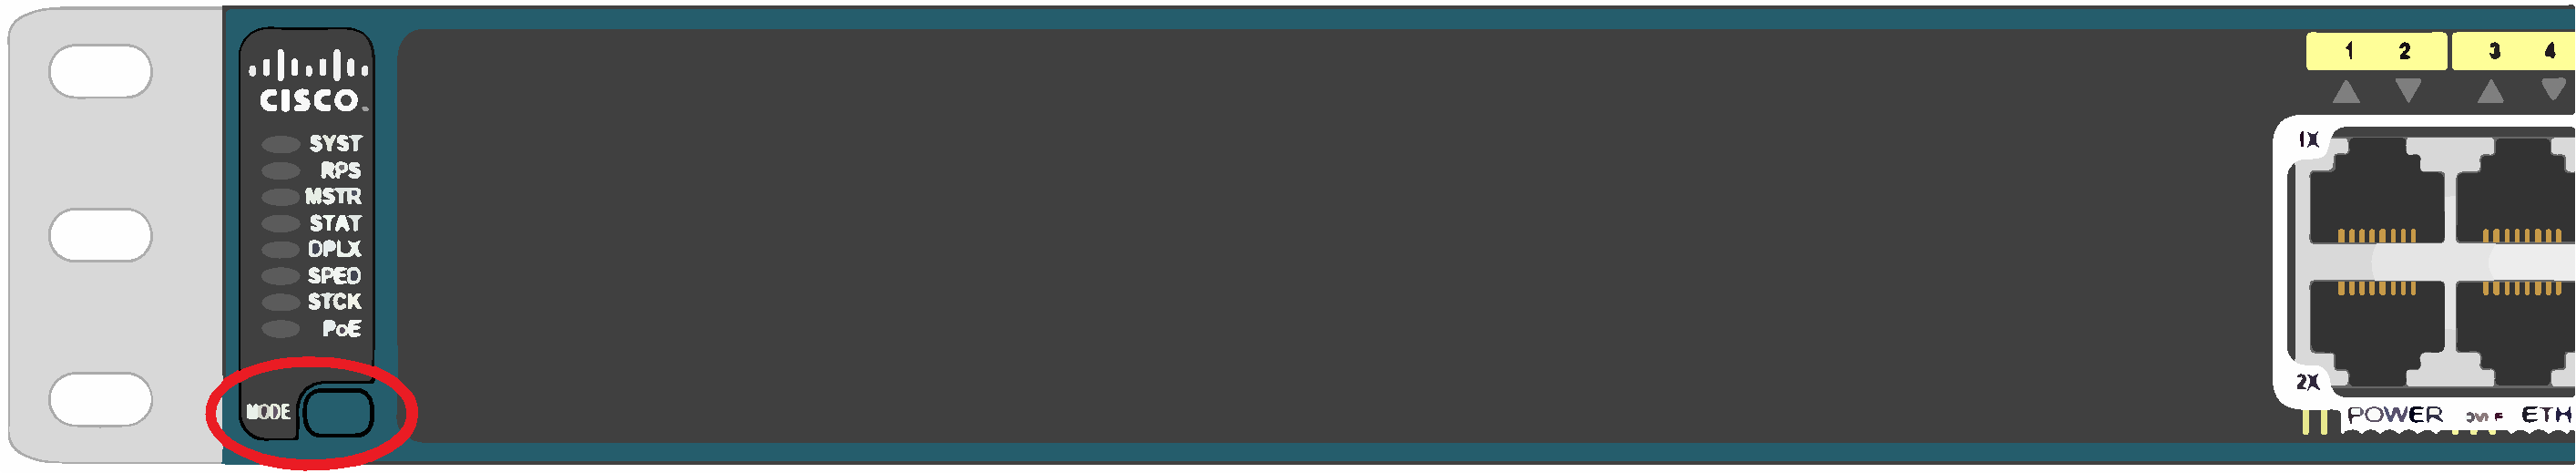
\includegraphics[width=\linewidth]{mode}
	\caption{To κουμπί mode, κάτω από τις φωτεινές ενδείξεις της συσκευής}\label{fig:mode}
\end{figure}

\subsection{Απαρίθμηση διεπαφών}
Σε κάθε διεπαφή/θύρα Ethernet μιας συσκευής Cisco έχει ανατεθεί μια ονομασία της μορφής:

\begin{center}
	\texttt{\large Porttype Χ/Υ/Z}\hspace*{0.5cm} ή\hspace*{0.5cm} \texttt{\large Porttype Χ/Z}
\end{center}

Ο αριθμός \texttt{Χ} αφορά το slot στο οποίο βρίσκεται η θύρα, το \texttt{Y} το subslot και το \texttt{Z} τον μοναδικό αριθμό της θύρας για το slot ή το slot/subslot που αυτή βρίσκεται. Το \texttt{Porttype} είναι λέξη κλειδί που δηλώνει την τεχνολογία της θύρας, η οποία μπορεί να είναι \texttt{FastEthernet} (\texttt{Fa}), \texttt{GigabitEthernet} (\texttt{Gi}) ή \texttt{TenGigabitEthernet}. Η ονομασία \texttt{Porttype Χ/Υ/Z} χρησιμοποιείται σε εντολές στο Cisco IOS προκειμένου να γίνει αναφορά στην αντίστοιχη θύρα της συσκευής.

\section{Βασικές εντολές του Cisco IOS}
Στην ενότητα αυτή παρατίθενται μερικές από τις πιο βασικές εντολές για τη διαχείριση οποιασδήποτε συσκευής Cisco. Οι εντολές αυτές, δηλαδή, μπορούν να εκτελεστούν τόσο σε δρομολογητές, όσο και σε μεταγωγείς Cisco.

\subsection{Μέθοδοι πρόσβασης στο CLI}
Ο χειρισμός μιας συσκευής Cisco πραγματοποιείται μέσω του CLI, η πρόσβαση στο οποίο μπορεί να γίνει με τις εξής μεθόδους:
\begin{itemize}
	\item [\textbf{Console}:] Η κονσόλα αποτελεί μια φυσική θύρα διαχείρισης, η οποία παρέχει πρόσβαση \textit{out-of-band} σε μια συσκευή Cisco. Ο όρος out-of-band αναφέρεται στη χρήση ενός αποκλειστικού καναλιού που προορίζεται για τη διαχείριση της συσκευής.
	\item [\textbf{SSH}:] Αν δεν υπάρχει φυσική πρόσβαση στο υπό διαχείριση μηχάνημα, είναι δυνατή η απομακρυσμένη σύνδεση σε αυτό μέσω του πρωτοκόλλου SSH, το οποίο παρέχει ασφαλή σύνδεση στο κέλυφος βασιζόμενο στη μέθοδο κρυπτογράφησης δημόσιου κλειδιού. Προϋπόθεση για τον συγκεκριμένο τύπο σύνδεσης είναι η ενεργοποίηση των απαραίτητων υπηρεσιών δικτύωσης, συμπεριλαμβανομένης μιας ενεργής διεπαφής με διεύθυνση IP. Η μέθοδος αυτή, όπως και οι ακόλουθες, αποκαλούνται \textit{in-band}, διότι χρησιμοποιούν ήδη υπάρχοντα κανάλια επικοινωνίας.
	\item [Telnet:] To πρωτόκολλο telnet επιτρέπει και αυτό απομακρυσμένη διαχείριση, όπως το SSH, με τη διαφορά ότι δεν υποστηρίζει κρυπτογράφηση, με αποτέλεσμα ευαίσθητες πληροφορίες όπως κωδικοί πρόσβασης να μεταδίδονται ως καθαρό κείμενο. Η χρήση του δεν συνίσταται.
	\item [AUX:] Η βοηθητική θύρα AUX (Auxilary port) επιτρέπει τη διαχείριση της συσκευής Cisco μέσω τηλεφωνικής γραμμής. Η συγκεκριμένη μέθοδος έχει πλέον εγκαταλειφθεί από τους διαχειριστές συστημάτων.
\end{itemize}

Στο πλαίσιο των εργαστηριακών ασκήσεων θα χρησιμοποιήσετε τη θύρα κονσόλας για τη σύνδεση στις δικτυακές συσκευές. Η σύνδεση στις κονσόλες πραγματοποιείται μέσω εικονικών σειριακών θυρών COM, κάθε μια εξ αυτών αντιστοιχεί σε μία συσκευή Usb-to-Serial, η οποία συνδέεται με USB στον υπολογιστή. Για να δείτε τις διαθέσιμες θύρες COM εκτελέστε από περιβάλλον Windows την εντολή \ip{devmgmt.msc} για να ανοίξετε τη Διαχείριση Συσκευών και αναπτύξτε τον κατάλογο Ports (COM and LPT).

Η σύνδεση στις εικονικές θύρες COM μπορεί να πραγματοποιηθεί με εξομοιωτές τερματικού, ένας εκ των οποίων είναι το PuTTY. Στην εικόνα \ref{fig:putty} φαίνονται οι ρυθμίσεις που πρέπει να εφαρμοστούν στο PuTTY για τη σύνδεση στην κονσόλα μιας συσκευής Cisco.

\begin{figure}[ht]
	\centering
	\includegraphics[width=\textwidth]{putty}
	\caption{Η απαραίτητη παραμετροποίηση του PuTTY}\label{fig:putty}
\end{figure}

Έχοντας επιβεβαιώσει την ορθότητα των ρυθμίσεων στο PuTTY και πατώντας το κουμπί Open, συνδέεστε στη συσκευή. Στο μαύρο κενό παράθυρο του PuTTY που εμφανίζεται θα πρέπει να πατήσετε μια φορά το \keystroke{Enter} για να εμφανιστεί η προτροπή του CLI. Πριν εμφανιστεί η προτροπή ενδέχεται να ζητηθεί κωδικός πρόσβασης.

\subsection{Λειτουργίες βοήθειας του IOS και διευκόλυνση πρόσβασης}
Το λειτουργικό σύστημα της Cisco διαθέτει δυο μορφές βοήθειας, την context-sensitive και τη βοήθεια συντακτικού ελέγχου. Η πρώτη λειτουργία επιτρέπει τη γρήγορη εύρεση των πιθανών λέξεων κλειδιών ή παραμέτρων που μπορεί να λάβει μια εντολή προσθέτοντας το σύμβολο \texttt{?}

\begin{CommandBox}
Router>`\textbf{ping ?}`
  WORD  Ping destination address or hostname
  ip    IP echo
  ipv6  IPv6 echo
Router>
\end{CommandBox}

Η βοήθεια συντακτικού ελέγχου αφορά την παράθεση πληροφοριών σε περίπτωση που εισαχθεί προς το CLI μη έγκυρη εντολή. Ο διερμηνέας εντολών ελέγχει την εντολή εισόδου από τα αριστερά προς τα δεξιά και σε περίπτωση που ανιχνευθεί κάποιο λάθος ενημερώνεται κατάλληλα ο χρήστης.

\begin{CommandBox}
Router>`\textbf{show ip intergace brief}`
                    ^
% Invalid input detected at '^' marker.

Router>
\end{CommandBox}

Ακόμη, το CLI δίνει τη δυνατότητα στον χρήστη να εκτελέσει μια εντολή με χρήση του ελάχιστου πλήθους χαρακτήρων που τη διακρίνουν μοναδικά. Για παράδειγμα, η εντολή \ip{show ip interface brief} εκτελείται και ως \ip{sh ip int br} και η εντολή \ip{copy running-config startup-config} είναι ισοδύναμη με την \ip{copy run start} και την \ip{copy r s}. 

H σύντμηση μπορεί να εφαρμοστεί σε οποιαδήποτε λέξη αποτελεί την εντολή, αρκεί να μην δημιουργείται ασάφεια, όταν μια σύντμηση ταυτίζεται με περισσότερες επιλογές. Για να προσδιορίσετε τις λέξεις με τις οποίες ταυτίζεται μια σύντμηση, μπορείτε να πληκτρολογήσετε την σύντμηση ακολουθούμενη από το \texttt{?}. Για παράδειγμα:

\begin{CommandBox}
Router>
Router>`\textbf{s?}`
show  ssh  
Router>`\textbf{sh?}`
show  
Router>`\textbf{sh ip int br}`
\end{CommandBox}

Τέλος, ο πίνακας \ref{tab:shortcuts} συνοψίζει τις βασικότερες συντομεύσεις πληκτρολογίου, οι οποίες μπορούν να διευκολύνουν την πρόσβαση στο CLI και την γρηγορότερη πληκτρολόγηση εντολών σε αυτό.
\begin{table}[ht]
	\centering\rowcolors{2}{lightgray}{white}
	\begin{MyTabularAuto}{Συντόμευση}{Αποτέλεσμα}
		\keystroke{Ctrl} + \keystroke{Shift} + \keystroke{6} & Ακύρωση εκτέλεσης εντολής (ping, domain-lookup κλπ)\\
		\keystroke{Ctrl} + \keystroke{P} ή \keystroke{$\ \uparrow\ $} & Εμφάνιση τελευταίας εντολής που δόθηκε\\
		\keystroke{Ctrl} + \keystroke{N} ή \keystroke{$\ \downarrow\ $} & Εμφάνιση προηγούμενων εντολών που δόθηκαν\\
		\keystroke{Ctrl} + \keystroke{A} & Μετακίνηση κέρσορα στην αρχή της γραμμής\\
		\keystroke{Ctrl} + \keystroke{E} & Μετακίνηση κέρσορα στο τέλος της γραμμής\\
		\keystroke{Esc } + \keystroke{B} & Μετακίνηση κέρσορα προς τα πίσω κατά μια λέξη\\
		\keystroke{Esc } + \keystroke{F} & Μετακίνηση κέρσορα προς τα εμπρός κατά μια λέξη\\
		\keystroke{Ctrl} + \keystroke{R} & Επανεμφάνιση μιας γραμμής\\
		\keystroke{Ctrl} + \keystroke{U} & Διαγραφή μιας γραμμής\\
		\keystroke{Ctrl} + \keystroke{W} & Διαγραφή μιας λέξης\\
		\keystroke{Ctrl} + \keystroke{Z} & Τερματισμός της κατάστασης ρυθμίσεων και επιστροφή στην κατάσταση EXEC\\
		\keystroke{Tab} & Ολοκλήρωση της πληκτρολόγησης μιας εντολής\\\hline
	\end{MyTabularAuto}
	\caption{Συντομεύσεις πληκτρολογίου για το CLI.}\label{tab:shortcuts}
\end{table}

\subsection{Μετάβαση μεταξύ καταστάσεων λειτουργίας}
Με την είσοδο σας στο CLI βρίσκεστε σε κατάσταση user EXEC. Για να μεταβείτε σε κατάσταση επαυξημένων δικαιωμάτων αρκεί να εκτελέσετε την εντολή \texttt{enable}, πληκτρολογώντας κατόπιν τον κατάλληλο κωδικό πρόσβασης, αν ζητηθεί:

\begin{CommandBox}
Router>`\textbf{enable}`
Password:
Router#
\end{CommandBox}

Αναγνωρίζετε πως είστε σε κατάσταση επαυξημένων δικαιωμάτων διακρίνοντας τη δίεση (\#) στην προτροπή, η οποία αντικαθιστά το σύμβολο συγκρίσεως (>) της κατάστασης user EXEC. Εξέρχεστε από την προνομιακή κατάσταση με την εντολή \texttt{disable}:

\begin{CommandBox}
Router#`\textbf{disable}`
Router>
\end{CommandBox}

Ευρισκόμενοι στην προνομιακή κατάσταση, μπορείτε να μεταβείτε στην κατάσταση καθολικής ρύθμισης (global configuration) με την εντολή \texttt{configure terminal}. Αναγνωρίζετε πως είστε σε κατάσταση καθολικής ρύθμισης παρατηρώντας την ένδειξη \texttt{config} στα αριστερά της δίεσης της προτροπής.

\begin{CommandBox}
Router#`\textbf{configure terminal}`
Router(config)#
\end{CommandBox}

Για να εξέλθετε από την κατάσταση ρυθμίσεων μπορείτε να δώσετε την εντολή \ip{exit} ή την εντολή \ip{end} ή τον συνδυασμό πλήκτρων \keystroke{Ctrl} + \keystroke{Z}.

\begin{CommandBox}
Router(config)#`\textbf{end}`
Router#
\end{CommandBox}

\subsection{Ασφαλίζοντας τις συσκευές Cisco}
Το Cisco IOS παρέχει μηχανισμούς ασφαλείας ώστε να περιορίζεται η πρόσβαση σε μη εξουσιοδοτημένα άτομα. Όπως φαίνεται και στο σχήμα \ref{fig:command-modes} (σελ. \pageref{fig:command-modes}) υπάρχει δυνατότητα ταυτοποίησης σε δυο στάδια, κατά την είσοδο στο user EXEC mode και για την είσοδο στην κατάσταση επαυξημένων δικαιωμάτων. 

\cautionbox{\bf Aπαγορεύεται ο ορισμός ή τροποποίηση των εξής κωδικών πρόσβασης για τα φυσικά μηχανήματα του εργαστηρίου: (1) \underline{κονσόλα} και (2) \underline{επαυξημένων δικαιωμάτων} . Οι εντολές αυτές μπορούν να εκτελεστούν με ασφάλεια στο Cisco Packet Tracer ή το GNS3.}

Ο ορισμός κωδικού κονσόλας γίνεται από την κατάσταση ρύθμισης κονσόλας ως εξής (όπου \texttt{\textit{cisco}} ο επιθυμητός κωδικός πρόσβασης). Η εντολή login χρησιμεύει ώστε ο οριζόμενος κωδικός να ζητηθεί από τον χρήστη στην επόμενη σύνδεση. \textbf{Μην εκτελέσετε τις εξής εντολές σε μηχάνημα Cisco του εργαστηρίου}.

\begin{CommandBox}
Router#`\textbf{configure terminal}`
Router(config)#`\textbf{line console 0}`
Router(config-line)#`\textbf{password} \textit{cisco}`
Router(config-line)#`\textbf{login}`
Router(config-line)#`\textbf{end}`
Router#
\end{CommandBox}

Ο ορισμός πρόσβασης για την πρόσβαση σε κατάσταση επαυξημένων δικαιωμάτων (privilege ή enable mode) μπορεί να γίνει με την εντολή \texttt{enable}. \textbf{Μην εκτελέσετε τις εξής εντολές σε μηχάνημα Cisco του εργαστηρίου}.

\begin{CommandBox}
Router(config)#`\textbf{enable secret} \textit{cisco}`
Router(config)#`\textbf{end}`
Router#
\end{CommandBox}

Το όρισμα \texttt{secret} αποθηκεύει τον επιθυμητό κωδικό πρόσβασης \texttt{cisco} κρυπτογραφημένο, κάτι το οποίο δεν γίνεται με την εντολή \texttt{password \textit{cisco}}, η οποία αποθηκεύει τον κωδικό πρόσβασης \texttt{cisco} ως καθαρό κείμενο (plaintext). 

\notebox{Οι εντολές που ακολουθούν μπορούν να εκτελεστούν με ασφάλεια στις συσκευές Cisco του εργαστηρίου.}

Για να ενεργοποιήσετε την κρυπτογράφηση στους κωδικούς πρόσβασης μπορείτε να εκτελέσετε την εντολή \texttt{service password-encryption}. Η εκτέλεση της εντολής έχει ως αποτέλεσμα οι κωδικοί να εμφανίζονται κρυπτογραφημένοι στις τρέχουσες ρυθμίσεις και στις ρυθμίσεις της NVRAM:

\begin{CommandBox}
Router(config)#`\textbf{service password-encryption}`
\end{CommandBox}

Κωδικοί πρόσβασης μπορούν να οριστούν και για την πρόσβαση μέσω των δικτυακών πρωτοκόλλων telnet και SSH. Τα πρωτόκολλα αυτά χρησιμοποιούν μια εικονική διεπαφή (Virtual TeletYpe - VTY) με εικονικές θύρες, οι οποίες είναι 6 στους δρομολογητές και 16 στους μεταγωγείς, με την αρίθμηση να ξεκινά από το 0. Κωδικός πρόσβασης για όλο το εύρος των εικονικών θυρών μπορεί να οριστεί με τις εξής εντολές:

\begin{CommandBox}
Router(config)#`\textbf{line vty 0 15}`
Router(config-line)#`\textbf{password} \textit{cisco}`
Router(config-line)#`\textbf{login}`
Router(config-line)#`\textbf{exit}`
Router(config)#
\end{CommandBox}

\subsection{Παραμετροποίηση τερματικού}

Οι καταστάσεις ρύθμισης κονσόλας και VTY παρέχουν διάφορες ρυθμίσεις, η ενεργοποίηση των οποίων συνίσταται διότι καθιστούν πιο άνετη την εργασία μέσω εξομοιωτή τερματικού, όπως το PuTTY. Από προεπιλογή, η συνεδρία με το τερματικό τερματίζεται όταν περάσει ένα χρονικό διάστημα κατά το οποίο ο χρήστης δεν πληκτρολογήσει κάτι. Αυτό το διάστημα ορίζεται με την εντολή \texttt{exec-timeout}, η οποία δέχεται ως όρισμα το εν λόγω διάστημα σε λεπτά. Δίνοντας 0 απενεργοποιείται το χρονικό όριο:

\begin{CommandBox}
Router(config)#`\textbf{line console 0} \textrm{\textit{ή για SSH/Telnet:}} \textbf{line vty 0 15}`
Router(config-line)#`\textbf{exec-timeout 0}`
Router(config-line)#`\textbf{exit}`
Router(config)#
\end{CommandBox}

Διάφορα γεγονότα, όπως η ενεργοποίηση/απενεργοποίηση μιας διεπαφής ή το πρόγραμμα αποσφαλμάτωσης, δημιουργούν μηνύματα syslog, τα οποία ανακατευθύνονται στην έξοδο της κονσόλας. Από προεπιλογή, τα μηνύματα προβάλλονται ασύγχρονα, με αποτέλεσμα να παρεμποδίζεται η πληκτρολόγηση εντολών στο τερματικό. Τα μηνύματα μπορούν να εμφανιστούν σύγχρονα, δηλαδή χωρίς να διακόπτεται η πληκτρολόγηση, με τις εντολές που ακολουθούν:

\begin{CommandBox}
Router(config)#`\textbf{line console 0} \textrm{\textit{ή για SSH/Telnet:}} \textbf{line vty 0 14}`
Router(config-line)#`\textbf{logging synchronous}`
Router(config-line)#`\textbf{exit}`
Router(config)#
\end{CommandBox}

\subsection{Αλλαγή hostname}
Κατά τη συνήθη πρακτική, ένας διαχειριστής αλλάζει το εργοστασιακό όνομα της συσκευής του, ώστε βλέποντας την προτροπή να γνωρίζει σε ποιο μηχάνημα δίνει εντολές. Συνήθως, το όνομα μιας συσκευής μπορεί να υποδηλώνει τη φυσική τοποθεσία της (πχ κτήριο, δωμάτιο και ράφι). Για να αλλάξετε το όνομα της συσκευής θα πρέπει να εκτελέσετε την εντολή \texttt{hostname x}, όπου \texttt{x} το νέο όνομα της συσκευής.

\begin{CommandBox}
Router#`\textbf{configure terminal}`
Router(config)#`\textbf{hostname R1}`
R1(config)#
\end{CommandBox}

Η μορφή των ονομάτων πρέπει να ακολουθεί τις οδηγίες του εγγράφου \href{https://tools.ietf.org/html/rfc1123}{RFC 1123}.

\subsection{Διαχείριση συστήματος αρχείων}

Ο πίνακας \ref{tab:dir} συνοψίζει τις βασικότερες εντολές για τον χειρισμό καταλόγων και αρχείων στο Cisco IOS. Πολλές από τις εντολές του πίνακα \ref{tab:dir} εμφανίζονται και σε συστήματα Unix και συντάσσονται με τον ίδιο τρόπο με αυτές.

\begin{CommandTableAuto}{Οι σημαντικότερες εντολές για χειρισμό καταλόγων στο Cisco IOS}{dir}
	\textbf{show filesystem} 		& Προβολή του συστήματος αρχείων της συσκευής\\
	\textbf{pwd} 			 		& Εμφάνιση τρέχοντος καταλόγου εργασίας.\\
	\textbf{dir} \textit{folder} 	& Εμφάνιση περιεχομένων ενός καταλόγου.\\
	\textbf{cd} \textit{folder} 	& Αλλαγή τρέχοντος καταλόγου εργασίας.\\
	\textbf{show} \textit{file} 	& Εμφάνιση πληροφοριών για συγκεκριμένο κατάλογο ή αρχείο.\\
	\textbf{delete} \textit{folder}	& Διαγραφή ενός αρχείου.\\
	\textbf{more} \textit{file}	& Προβολή περιεχομένων ενός αρχείου.
\end{CommandTableAuto}

\subsection{Προβολή πληροφοριών}
Με την εντολή \texttt{show interface} μπορείτε να προβάλλετε αναλυτικές λεπτομέρειες για όλες τις δικτυακές διεπαφές της συσκευής που χειρίζεστε.

\begin{CommandBox}
Router>`\textbf{show interface}`
\end{CommandBox}
Μπορείτε να περιορίσετε τα αποτελέσματα της εντολής ορίζοντας το όνομα της διεπαφής που σας ενδιαφέρει. Για παράδειγμα, η εντολή \texttt{show interface GigabitEthernet1/0/1} θα εμφανίσει πληροφορίες για τη διεπαφή \texttt{GigabitEthernet1/0/1}.

\begin{CommandBox}
Router>`\textbf{show interface GigabitEthernet1/0/1}`
\end{CommandBox}

Πολύ χρήσιμη είναι η εντολή \texttt{show ip interface brief}, η οποία προβάλλει μια σύνοψη της κατάστασης όλων των διεπαφών της συσκευής. Συγκεκριμένα, για κάθε διεπαφή διακρίνετε αν είναι ενεργοποιημένη και αν έχει αντιστοιχηθεί διεύθυνση IP σε αυτήν.

\begin{CommandBox}
Router>`\textbf{show ip interface brief}`
Interface           IP-Address   OK? Method Status                Protocol 
GigabitEthernet0/0  unassigned   YES unset  administratively down down 
GigabitEthernet0/1  unassigned   YES unset  administratively down down 
GigabitEthernet0/2  unassigned   YES unset  administratively down down 
Vlan1               unassigned   YES unset  administratively down down
Router>
\end{CommandBox}

Τέλος, με την εντολή \texttt{show version} μπορείτε να προβάλλετε πληροφορίες που αφορούν την δικτυακή σας συσκευή, όπως έκδοση IOS, χαρακτηριστικά του hardware κ.λ.π.

\begin{CommandBox}
Router>`\textbf{show version}`
\end{CommandBox}

\subsection{Διασωλήνωση}
Με την χρήση της διασωλήνωσης (\texttt{|}) μπορείτε να φιλτράρετε τα αποτελέσματα μιας εντολής. Μερικά παραδείγματα παρατίθενται στον πίνακα \ref{tab:pipeline}.

\begin{CommandTable*}{Ενδεικτικές εφαρμογές της διασωλήνωσης στο CLI}{pipeline}{10cm}{7cm}
	Router>\textbf{show running-config | ?} & Εμφάνιση όλων των δυνατών επιλογών για την εντολή διασωλήνωσης, όπως \texttt{begin}, \texttt{include}, \texttt{exclude} κ.τ.λ. \\[0.25cm]
	Router>\textbf{show run | begin interface} & Εμφάνιση τρέχουσας κατάστασης ρυθμίσεων ξεκινώντας από τις ρυθμίσεις των διεπαφών.\\[0.25cm]
	Router>\textbf{show ip route | include 192.168.3.32} & Εμφάνιση όλων των καταχωρήσεων του πίνακα δρομολόγησης, οι οποίες περιλαμβάνουν την διεύθυνση \texttt{192.168.3.32}.
\end{CommandTable*}

\subsection{MOTD banner}

Συνήθης πρακτική παραμετροποίησης των συσκευών Cisco σε παραγωγικό περιβάλλον είναι ο ορισμός μηνυμάτων νομικού περιεχομένου, τα οποία προειδοποιούν έναν χρήστη για τις συνέπειες του νόμου, σε περίπτωση που κάποιος μη εξουσιοδοτημένος χρήστης συνδεθεί σε μια συσκευή ή για το γεγονός ότι η πρόσβασή τους καταγράφεται.

Με την εντολή \texttt{banner motd} μπορείτε να ορίσετε το μήνυμα-της-ημέρας (MOTD - Message Of The Day), το οποίο προβάλλεται όταν ένας χρήστης συνδέεται σε ένα μηχάνημα Cisco. Η εντολή είναι διαθέσιμη από την κατάσταση ρυθμίσεων και η γενική της μορφή είναι η εξής:

\begin{CommandBox}
Router(config)#`\textbf{banner motd} \textit{delimiter message delimiter}`
\end{CommandBox}

Όπου \texttt{message}, το μήνυμα που επιθυμείτε να προβάλλεται στον χρήστη και \texttt{delimiter} ένας χαρακτήρας, ο οποίος δηλώνει την έναρξη και το τέλος του μηνύματος και δεν περιέχεται μέσα στο μήνυμα. Ένα παράδειγμα εκτέλεσης φαίνεται παρακάτω:

\begin{CommandBox}
Router(config)#`\textbf{banner motd \$\#\#\#\#\#\#\#\#\#\#\#\#\#\#}`
Enter TEXT message.  End with the character '$'.
`\textbf{You are connected to Cisco 2921\\
Unauthorized access to this system is\\
forbidden and will be prosecuted by law.\\
\#\#\#\#\#\#\#\#\#\#\#\#\#\#\$}`

Router(config)#
\end{CommandBox}

Μπορείτε να δημιουργήσετε banner πολλών γραμμών, πατώντας \keystroke{Enter} πριν πληκτρολογήσετε τον δεύτερο \texttt{delimeter} και να ολοκληρωθεί το μήνυμα του banner.

Ενδεικτικά, το ακόλουθο κείμενο είναι το banner που χρησιμοποιεί η British Telekom για την προστασία των συσκευών της:

\begin{quote}\ttfamily\singlespacing
	CC\\
	"British Telecommunication plc"\\
	WARNING: You have accessed a computer managed by BT. You are required
	to have authorisation from BT before you proceed and you are strictly
	limited to the use set out within that authorisation.
	
	Unauthorised access to or misuse of this system is prohibited and con\\stitutes an offence under the Computer Misuse Act 1990.
	
	If you disclose any information obtained through this system without
	authority BT may take legal action against you.
	
	If you are authorised to use this computer enter your authentication
	details otherwise terminate this connection now.
\end{quote}
 
\subsection{Εντολή no}
Με την γενικής χρήσης εντολή \texttt{no} μπορείτε να ακυρώσετε την ενέργεια που προκαλεί η εντολή που την ακολουθεί. Για παράδειγμα, με την εντολή \texttt{no ip domain-lookup} μπορείτε να απενεργοποιήσετε τη λειτουργία αναζήτησης ονομάτων τομέα (domain names).\footnote{Προτείνεται η εκτέλεση της \texttt{no ip domain-lookup} όταν δεν εργάζεστε με το πρωτόκολλο DNS, ώστε να αποφύγετε ανεπιθύμητες αναζητήσεις ονομάτων τομέα.}

\begin{CommandBox}
Router(config)#`\textbf{no ip domain-lookup}`
\end{CommandBox}

Αντίστοιχα, μπορείτε να απενεργοποιήσετε το MOTD banner ως εξής: 

\begin{CommandBox}
Router(config)#`\textbf{no banner motd}`
\end{CommandBox}

\end{document}
